\chapter{Guideline d'annotation et extraction multimodale}
\label{chap:extraction}

\section{Introduction}\label{sec:c3-3-1}

Pour extraire automatiquement des informations cliniques de dossiers médicaux, il faut d'abord définir précisément ce qu'il faut extraire. Ce mémoire a été réalisé au sein de l'IHU PROMETHEUS (\emph{PRecisiOn MedicinE for healTHcare associatEd and commUnity acquired Sepsis}), dans le Work Package 6, qui étudie le sepsis sous ses différents aspects. Il fait suite au cadre KG-EDS (\emph{Knowledge Graph for Early Diagnosis of Sepsis})~\cite{kgeds}, dont l'extraction reposait sur l'apprentissage en contexte, sans schéma d'annotation formalisé ni corpus annoté.

Ce chapitre réunit les deux éléments qui produisent le graphe de connaissances à partir des dossiers. Le premier est le \emph{TRACE-Sepsis Annotation Guideline}, un guide propre au sepsis qui fixe les concepts cliniques à représenter, les relations permises entre eux et la conduite à tenir face à la négation, à la temporalité, aux valeurs chiffrées et aux cas ambigus. Le Pr Nicholas Heming, médecin réanimateur spécialiste du sepsis, l'a validé. Le second est le pipeline d'extraction multimodale, qui fait lire les pages scannées par un grand modèle de langage multimodal et construit ses consignes à partir de ce même guideline. Le modèle et l'annotatrice du Gold Standard, présenté au chapitre~\ref{chap:donnees-gold}, suivent ainsi les mêmes règles.

Le chapitre décrit d'abord le corpus clinique et les règles de protection des données qui l'encadrent (section~\ref{sec:c3-3-2}), puis le guideline et ses fondements (section~\ref{sec:c3-3-3}), le schéma d'entités (section~\ref{sec:c3-3-4}), le schéma de relations (section~\ref{sec:c3-3-5}) et les règles d'annotation (section~\ref{sec:c3-3-6}). Il présente ensuite le pipeline d'extraction : son architecture (section~\ref{sec:c4-archi}), la préparation des dossiers (section~\ref{sec:c4-preparation}), la construction des consignes (section~\ref{sec:c4-prompt}), les deux modèles comparés (section~\ref{sec:c4-modeles}), l'extraction des entités et des relations (sections~\ref{sec:c4-entites} et~\ref{sec:c4-relations}), la mise en forme des sorties (section~\ref{sec:c4-postproc}) et les corrections apprises (section~\ref{sec:c4-appris}). Il se termine par les critères de choix du modèle (section~\ref{sec:c4-selection}).

% ============================================================
\section{Corpus clinique}\label{sec:c3-3-2}

\subsection{Nature et origine des données}\label{sec:c3-3-2-1}

Les documents étudiés sont des dossiers médicaux numérisés de patients pris en charge pour un sepsis. Ils proviennent de la cohorte APROCCHSS (1\,240 patients), constituée lors de l’essai multicentrique du même nom chez des patients en choc septique~\cite{annane2018aprocchss}. L’Assistance Publique -- Hôpitaux de Paris (AP-HP) les a mis à disposition dans le cadre du Work Package 6 de l’IHU PROMETHEUS. Ils couvrent les années 2008 à 2015 et viennent du service de médecine intensive--réanimation de l’Hôpital Raymond-Poincaré (AP-HP).

Ces dossiers n’ont rien d’une base de données structurée, où chaque information aurait son champ. Ils ont été rédigés au fil de la prise en charge et mêlent observations médicales, paramètres physiologiques, résultats biologiques et microbiologiques, prescriptions, comptes rendus d’examens, diagnostics et notes d’évolution. La plupart sont antérieurs à la définition Sepsis-3 de 2016~\cite{singer2016third} et emploient donc le vocabulaire de Sepsis-2~\cite{levy2003sccm}, comme « sepsis sévère ».

Une même information revient souvent à plusieurs endroits, sous une forme plus ou moins précise. Une suspicion d’infection peut ainsi apparaître dans l’observation d’entrée, être précisée par une imagerie, puis confirmée par un prélèvement. Une phrase ou une page isolée ne suffit donc pas toujours à comprendre le contexte clinique. C’est pourquoi \textbf{le dossier patient est l’unité clinique de référence} dans ce travail, même si certaines opérations se font page par page.

\subsection{Hétérogénéité documentaire}\label{sec:c3-3-2-2}

Les dossiers sont des fichiers PDF obtenus par numérisation de documents papier. D’une page à l’autre, la mise en page, la densité du texte, l’orientation et la qualité du scan changent. Une partie de l’information est rédigée en texte libre, une autre est rangée dans des tableaux ou des formulaires. Ailleurs, des résultats sont simplement alignés sur une même ligne : le nom d’un paramètre, sa valeur et son unité, parfois suivis des valeurs normales du laboratoire (par exemple « Leucocytes 40,8 4,0--10,0 G/L »).

La variabilité est aussi sémantique. Un même fait peut être écrit de plusieurs façons, abrégé, ou complété sur une autre page. Certains éléments n’ont de sens qu’avec leur contexte : une valeur biologique doit être rattachée à son biomarqueur et à son unité, un traitement à sa posologie, à sa voie d’administration ou à sa date. Une information donnée sur une page peut enfin être confirmée, précisée ou contredite plus loin, ce qui conforte le choix du dossier comme unité de représentation.

Comme il s’agit de scans, ces documents ne se comportent pas comme des textes nativement numériques : la disposition de la page, la position relative des informations et la qualité de l’image influencent l’extraction. C’est l’une des raisons du recours à des modèles vision-langage, qui lisent directement les pages scannées. Dans TRACE, le document est traité comme une source multimodale, et non comme une image qu’il faudrait d’abord convertir en texte par OCR.

\subsection{Taille et description du corpus}\label{sec:c3-3-2-3}

Le corpus final compte \textbf{246 dossiers médicaux}, réunis progressivement au rythme des mises à disposition. \textbf{49 dossiers}, soit environ 20\,\% du corpus, ont été retenus pour construire la référence annotée. Ils représentent \textbf{291 pages}, de 4 à 12 pages par dossier (5,9 en moyenne). Les autres dossiers serviront aux étapes ultérieures d’extraction et d’exploitation. Le tableau~\ref{tab:c3-3-1} résume ces caractéristiques.

\begin{table}[H]
\centering
\caption{Caractéristiques du corpus}\label{tab:c3-3-1}
\small
\begin{tabular}{>{\raggedright\arraybackslash}p{0.404\linewidth}>{\raggedright\arraybackslash}p{0.231\linewidth}>{\raggedright\arraybackslash}p{0.231\linewidth}}
\toprule
\textbf{Caractéristique} & \textbf{Corpus complet} & \textbf{Sous-corpus de référence} \\
\midrule
Nombre de dossiers & 246 & 49 ($\approx$ 20\,\%) \\
Nombre total de pages & \acompleter{à compléter} & 291 \\
Pages par dossier (min--max) & \acompleter{à compléter} & 4--12 (moyenne : 5,9) \\
Période couverte & 2008--2015 & 2008--2015 \\
Établissement / service & Médecine intensive--réanimation, Hôpital Raymond-Poincaré (AP-HP) & Médecine intensive--réanimation, Hôpital Raymond-Poincaré (AP-HP) \\
\bottomrule
\end{tabular}
\end{table}

\subsection{Protection des données et cadre réglementaire}\label{sec:c3-3-2-4}

Les dossiers contiennent des données de santé. Leur confidentialité a donc été prise en compte dès la préparation du corpus, en limitant le traitement à ce qui était nécessaire aux objectifs scientifiques.

Une première pseudonymisation a été faite à la main par l'AP-HP, avant la mise à disposition. Les comptes rendus ont été imprimés et le nom et le prénom du patient partiellement masqués au stylo noir : quelques lettres ont été recouvertes, sans que l'identité soit entièrement effacée. Les pages ont ensuite été scannées et regroupées en fichiers PDF, que nous avons récupérés sur l'intranet de l'AP-HP. C'est pour cette raison que les dossiers n'ont pas de couche texte : l'information n'est accessible qu'à travers l'image des pages (section~\ref{sec:c3-3-2-2}).

Ce masquage ne concerne que le nom du patient, et quelques lettres peuvent rester lisibles ; lorsque le nom est répété ailleurs dans le compte rendu, il est effacé par la seconde pseudonymisation décrite ci-dessous. Les dates, comme la date de naissance ou les dates d'entrée et de sortie, ont en revanche été conservées, car elles sont nécessaires pour reconstituer la chronologie de la prise en charge. Au sens du RGPD, ces données sont donc pseudonymisées et non anonymisées : elles restent des données à caractère personnel et ont été traitées comme telles.

Une seconde pseudonymisation, automatique, a été appliquée aux textes transcrits des pages et aux annotations, à la demande du médecin référent. Elle repose sur des règles explicites : effacement des noms du patient restés lisibles hors de l'en-tête, de ceux de ses proches et des noms de médecins figurant dans l'en-tête des comptes rendus, ainsi que des numéros de téléphone. Chaque caractère effacé est remplacé par un caractère de substitution, ce qui conserve la longueur du texte et donc les positions des annotations. Les outils de désidentification automatique fondés sur l'apprentissage, qui existent pour les dossiers cliniques en français~\cite{elazzouzi2024}, n'ont pas été utilisés.

Les informations qui identifient directement un patient ne sont ni annotées ni extraites : le schéma se limite aux éléments utiles pour représenter le contexte clinique. Ce choix applique le principe de minimisation de l'article~5 du RGPD (Règlement (UE) 2016/679~\cite{rgpd2016}), selon lequel les données doivent être adéquates, pertinentes et limitées à ce qui est nécessaire aux finalités du traitement. Le même article pose aussi les principes de limitation des finalités, selon lequel les données ne servent qu'aux objectifs pour lesquels elles ont été collectées, et d'intégrité et de confidentialité, qui exige de les protéger contre tout accès ou usage non autorisé. L'article~89 précise comment appliquer ces principes lorsque les données servent à la recherche scientifique : il impose des garanties appropriées pour les droits et libertés des personnes concernées, sous la forme de mesures techniques et organisationnelles qui assurent notamment le respect de la minimisation. La pseudonymisation fait partie de ces mesures, dès lors qu'elle permet encore d'atteindre les objectifs de la recherche ; et lorsque ces objectifs peuvent être atteints avec des données qui ne permettent plus d'identifier les personnes, c'est cette solution qui doit être retenue. Les deux pseudonymisations décrites ci-dessus et l'exclusion des données directement identifiantes constituent les garanties mises en place dans ce travail.

Le format des documents impose une précaution supplémentaire. Dans un scan, une information sensible peut se trouver dans l'image même de la page, indépendamment de tout texte. La protection des données doit donc porter sur le document visuel entier. C'est d'autant plus important dans ce travail que les modèles multimodaux lisent directement les pages : la protection des données accompagne tout le protocole, de la préparation du corpus jusqu'à l'évaluation.

Les deux modèles multimodaux utilisés dans ce travail ont été mis en œuvre dans des conditions compatibles avec le RGPD. Qwen2.5-VL~\cite{bai2025qwen25vl} a été exécuté localement, sur un GPU de l'université, de sorte que les images des dossiers traitées par ce modèle n'ont pas quitté l'infrastructure universitaire. Mistral Small~4~\cite{mistralsmall4} a été utilisé par l'intermédiaire de l'offre payante de l'API de Mistral AI, société française établie dans l'Union européenne et donc directement soumise au RGPD. Son utilisation a été paramétrée de façon à limiter au strict nécessaire ce qui est transmis et ce qui peut en être fait :
\begin{itemize}
  \item \textbf{aucune réutilisation pour l'entraînement} : l'option d'amélioration des modèles à partir des données des utilisateurs (\emph{Anonymous improvement data}) a été désactivée dans les paramètres de confidentialité de la console d'administration. Les pages envoyées ne servent donc qu'à produire la réponse demandée, et jamais à entraîner les modèles de Mistral AI~\cite{mistral_retention} ;
  \item \textbf{aucun stockage de notre fait} : seul le point d'accès standard de génération (\texttt{https://api.mistral.ai/v1/chat/completions}) a été appelé. Il traite chaque requête de façon indépendante, sans historique de conversation ; les services qui stockent des données sur les serveurs de Mistral AI, comme les agents, les fichiers ou l'affinage de modèles (\emph{fine-tuning}), n'ont pas été utilisés ;
  \item \textbf{un hébergement européen} : les données de ce point d'accès sont traitées par défaut dans des centres de données situés dans l'Union européenne ;
  \item \textbf{des données déjà pseudonymisées} : l'API ne reçoit que les images des pages, déjà pseudonymisées à la main par l'AP-HP, leur transcription et les consignes d'extraction, qui contiennent trois pages annotées d'autres dossiers issues de ces mêmes documents pseudonymisés. Aucune donnée directement identifiante n'est demandée au modèle ni extraite par lui ;
  \item \textbf{un accès protégé} : la clé d'accès à l'API est fournie au moment de l'exécution et n'est jamais enregistrée dans le code ni dans les fichiers du projet.
\end{itemize}
Ces précautions appliquent directement les principes de l'article~5 : la limitation des finalités, puisque les données ne servent qu'à l'extraction, et l'intégrité et la confidentialité, puisque les données restent dans l'Union européenne, chez un prestataire soumis au RGPD, sans réutilisation ni stockage durable de notre fait.

\section{Le TRACE-Sepsis Annotation Guideline}\label{sec:c3-3-3}

\subsection{Motivation}\label{sec:c3-3-3-1}

Dans un dossier clinique, une même expression peut se lire de plusieurs façons. Selon le contexte, une manifestation relève d’un symptôme, d’un paramètre physiologique ou d’une défaillance d’organe. Deux concepts cités côte à côte ne sont pas pour autant liés. Sans règles écrites, chaque annotateur trancherait à sa manière ; il fallait donc formaliser ces décisions pour obtenir une annotation homogène et reproductible.

Le TRACE-Sepsis Annotation Guideline, dans sa version 2.0 validée par le médecin, répond à ce besoin. Il traite deux questions. La première, \emph{quelles informations représenter ?}, relève du schéma d’entités et de relations (sections~\ref{sec:c3-3-4} et~\ref{sec:c3-3-5}). La seconde, \emph{selon quelles règles les annoter ?}, relève des règles d’annotation (section~\ref{sec:c3-3-6}).

\subsection{Principes de conception}\label{sec:c3-3-3-2}

Quatre principes ont orienté sa rédaction.

\begin{itemize}
  \item \textbf{Ancrage documentaire.} Ne sont représentées que les informations réellement présentes dans le dossier. Aucune entité ni relation n’est ajoutée à partir de connaissances médicales extérieures, même plausibles : un antibiotique habituellement prescrit contre une infection ne suffit pas à annoter le diagnostic correspondant. C’est sur ce principe que repose l’évaluation des hallucinations, puisqu’une information sans preuve dans le document ne doit pas figurer dans le Gold Standard.
  \item \textbf{Séparation entre mention et normalisation.} La mention est conservée telle qu’elle est écrite, pour garder le lien avec la preuve ; sa normalisation est traitée à part.
  \item \textbf{Cohérence relationnelle.} Une relation doit être justifiée par le dossier et respecter les types d’entités autorisés pour son sujet et pour son objet.
  \item \textbf{Dimension longitudinale.} Des informations relatives à des moments différents du parcours ne sont pas fusionnées sans tenir compte de leur date.
\end{itemize}

\subsection{Fondements cliniques}\label{sec:c3-3-3-3}

Le guideline s’appuie sur les références qui font autorité dans le sepsis : les définitions Sepsis-2~\cite{levy2003sccm} et Sepsis-3~\cite{singer2016third}, les recommandations de la Surviving Sepsis Campaign~\cite{evans2021ssc}, le score SOFA~\cite{vincent1996sofa}, les recommandations KDIGO sur l’insuffisance rénale aiguë~\cite{kdigo2012aki} et, pour la microbiologie, les tables EUCAST en version 14.0~\cite{eucast}. Ces références cadrent la définition des concepts et une partie des règles de typage. Le vocabulaire de Sepsis-2 présent dans les dossiers (« sepsis sévère ») est conservé tel quel : on annote le diagnostic écrit, sans le traduire dans les termes de Sepsis-3.

Le guideline n’est pas pour autant un outil diagnostique. Il dit comment représenter une information quand elle est écrite, et non comment déduire un diagnostic à partir des recommandations. La nuance compte pour l’étude des hallucinations : une information médicalement juste mais absente du dossier n’a pas sa place dans le Gold Standard.

\subsection{Élaboration et validation du guideline}\label{sec:c3-3-3-4}

Une première version du guideline a été rédigée avant la campagne d’annotation. En l’appliquant aux premiers dossiers, plusieurs points se sont révélés insuffisamment précis : catégories dont les frontières se recouvrent, informations qui pouvaient relever de deux types, conditions d’usage de certaines relations, variantes d’écriture d’un même concept (« CRP » et « C.R.P. »). Ces difficultés ont été reprises avec le médecin référent, et le guideline a été révisé jusqu’à sa version finale, la version 2.0.

La validation médicale a été menée avec le Pr Nicholas Heming, professeur de médecine intensive--réanimation à l’Hôpital Raymond-Poincaré (AP-HP) et à l’Université Versailles-Saint-Quentin-en-Yvelines (Université Paris-Saclay), dont les recherches portent principalement sur le sepsis et le choc septique. Elle s’est déroulée en plusieurs séances de travail, pour un total d’environ cinq heures. Le médecin a examiné les catégories d’entités, leurs vocabulaires, les relations autorisées et les règles d’annotation, en particulier les cas où seule une décision clinique permet de choisir entre deux catégories. Ses remarques ont notamment conduit à restreindre les diagnostics autorisés à ceux qui concernent le sepsis et à ajuster les relations, pour aboutir à un schéma de 34 relations.

La version 2.0 précise aussi deux points qui posaient souvent problème. Un diagnostic de la liste autorisée reste un \entite{LABEL\_NOSOLOGIQUE}, qu’il concerne l’hospitalisation en cours ou un épisode antérieur ; tout autre antécédent est une \entite{COMORBIDITE\_ANTECEDENT}. Un \entite{FOYER\_INFECTIEUX} sert uniquement à localiser un diagnostic, auquel il est rattaché par la relation \emph{label\_nosologique\_a\_pour\_foyer}. C’est cette version validée par le médecin qui a servi à produire et à contrôler les annotations du Gold Standard.

\section{Schéma d’entités}\label{sec:c3-3-4}

\subsection{Organisation des entités par dimension clinique}\label{sec:c3-3-4-1}

Le schéma d’annotation sert à passer du contenu des dossiers à une connaissance structurée. Il comprend deux volets : les entités, qui représentent les informations cliniques, et les relations, qui les relient. Il ne s’agit pas seulement de repérer des termes médicaux, mais de reconstituer de façon ordonnée le parcours clinique du patient.

Le schéma compte \textbf{20 types d’entités cliniques}, plus une catégorie technique de métadonnées (section~\ref{sec:c3-3-4-2}). Le tableau~\ref{tab:c3-3-2} les regroupe selon les grandes dimensions du dossier. Chaque type dispose d’un vocabulaire contrôlé et d’attributs propres : \entite{LABEL\_NOSOLOGIQUE} admet par exemple 23 valeurs (sepsis, choc septique, SDRA, IRA, pneumopathie…), et \entite{BIOMARQUEUR} porte une valeur, une unité et une direction d’évolution (augmentation, diminution, stable, normalisation, inconnue).

\begingroup\small
\begin{longtable}{>{\raggedright\arraybackslash}p{0.192\linewidth}>{\raggedright\arraybackslash}p{0.260\linewidth}>{\raggedright\arraybackslash}p{0.413\linewidth}}
\caption{Types d’entités du schéma TRACE-Sepsis, par dimension clinique}\label{tab:c3-3-2}\\
\toprule
\textbf{Dimension} & \textbf{Type d’entité} & \textbf{Contenu représenté} \\
\midrule
\endfirsthead
\multicolumn{3}{l}{\emph{Tableau~\ref{tab:c3-3-2} (suite)}}\\
\toprule
\textbf{Dimension} & \textbf{Type d’entité} & \textbf{Contenu représenté} \\
\midrule
\endhead
\midrule
\multicolumn{3}{r}{\emph{Suite page suivante}}\\
\endfoot
\bottomrule
\endlastfoot
Patient et diagnostic & \entite{DONNEE\_\allowbreak{}PATIENT} & Le patient et ses données démographiques non identifiantes (âge, sexe, poids, taille, IMC), relevées à l’admission \\
 & \entite{LABEL\_\allowbreak{}NOSOLOGIQUE} & Diagnostic écrit dans le dossier et figurant dans la liste autorisée (sepsis, choc septique, pneumopathie…), y compris pour un épisode antérieur \\
Évaluation clinique et physiologique & \entite{SIGNE\_\allowbreak{}VITAL} & Paramètre physiologique, hémodynamique ou ventilatoire mesuré (valeur, unité, horodatage) \\
 & \entite{SCORE\_\allowbreak{}SOFA}, \entite{SCORE\_\allowbreak{}qSOFA} & Scores de dysfonction d’organes et de dépistage du sepsis \\
 & \entite{SCORE\_\allowbreak{}NEUROLOGIQUE} & Score neurologique rapporté (Glasgow, RASS, FOUR, MMS, testing musculaire) \\
 & \entite{STADE\_\allowbreak{}IRA} & Stade 1 à 3 d’insuffisance rénale aiguë (classification KDIGO 2012) \\
Infection et biologie & \entite{BIOMARQUEUR} & Résultat biologique quantitatif, avec valeur, unité et direction d’évolution (ex. CRP 245 mg/L) \\
 & \entite{FOYER\_\allowbreak{}INFECTIEUX} & Localisation d’un diagnostic infectieux (organe, région, site) \\
 & \entite{MICRO\_\allowbreak{}ORGANISME} & Agent microbiologique identifié \\
Manifestations et atteintes & \entite{SYMPTOME} & Manifestation qualitative observée ou rapportée \\
 & \entite{DEFAILLANCE\_\allowbreak{}ORGANE} & Dysfonction ou défaillance d’un organe \\
Prise en charge thérapeutique & \entite{TRAITEMENT} & Médicament ou intervention thérapeutique \\
 & \entite{POSOLOGIE} & Dose, schéma horaire, voie, débit et durée d’administration \\
Terrain et contexte & \entite{COMORBIDITE\_\allowbreak{}ANTECEDENT} & Pathologie préexistante ou antécédent hors liste des diagnostics \\
 & \entite{CONTEXTE\_\allowbreak{}ACQUISITION} & Mode d’acquisition (communautaire, nosocomiale, associée aux soins…) et expositions \\
Temporalité et parcours de soins & \entite{EVENEMENT\_\allowbreak{}TEMPOREL} & Événement daté (admission, administration, transfert…) \\
 & \entite{EVOLUTION\_\allowbreak{}PRONOSTIC} & Évolution clinique et devenir du patient \\
 & \entite{SERVICE\_\allowbreak{}MEDICAL} & Type de service de prise en charge (réanimation, urgences, SSR…), sans le nom de l’établissement \\
Examens & \entite{IMAGERIE\_\allowbreak{}PROCEDURE} & Examen d’imagerie ou procédure diagnostique (type, région, résultat, horodatage) \\
\end{longtable}
\endgroup

Plusieurs distinctions structurent ce schéma. \entite{DONNEE\_PATIENT} et \entite{LABEL\_NOSOLOGIQUE} sont séparés pour ne pas confondre le patient avec les pathologies qui lui sont attribuées. Le contexte infectieux est découpé en trois concepts : une CRP élevée, un foyer pulmonaire et un germe isolé sont trois informations distinctes, même quand elles décrivent le même épisode. Un \entite{SYMPTOME} n’est ni un diagnostic, ni une défaillance d’organe, ni un résultat biologique. Enfin, séparer \entite{TRAITEMENT} et \entite{POSOLOGIE} permettra de distinguer plusieurs erreurs : mauvais médicament, mauvaise dose, ou mauvais lien entre le traitement et le patient. La posologie est une entité et non un simple attribut, pour trois raisons : elle a une structure interne (dose, unité, schéma horaire), une temporalité propre (une dose peut être ajustée sans que le médicament change), et des notations variées (« 1-0-1 », « 1 amp/8h ») qu’il faut pouvoir décomposer.

\subsection{Métadonnées de traçabilité}\label{sec:c3-3-4-2}

Le guideline prévoit aussi des métadonnées techniques : identifiant de l’entité, page d’origine, boîte englobante (\emph{bbox}) situant l’information sur la page, confiance visuelle et confiance globale, type d’inférence et indicateur de négation (\emph{nie}). Elles ne décrivent aucune connaissance médicale. Leur rôle est de relier chaque information structurée à l’endroit du document d’où elle vient, ce qui est précieux pour repérer et analyser les hallucinations.

\section{Schéma de relations}\label{sec:c3-3-5}

\subsection{Principe et familles de relations}\label{sec:c3-3-5-1}

Repérer les entités ne suffit pas à rendre compte de l’organisation d’un dossier. Savoir qu’un antibiotique, un patient et un germe sont mentionnés ne dit pas si l’antibiotique a été donné au patient, ni s’il visait ce germe. TRACE-Sepsis définit donc un ensemble fermé de relations orientées, de la forme \emph{sujet $\rightarrow$ relation $\rightarrow$ objet}. Chaque type de relation a un domaine (\emph{domain}) et une portée (\emph{range}) autorisés.

La version 2.0 du guideline comporte \textbf{34 signatures relationnelles}. Leur liste et leurs couples domaine--portée sont figés, pour qu’aucune normalisation ni correction ne modifie la structure du schéma. Le tableau~\ref{tab:c3-3-3} les regroupe en huit familles ; la liste complète figure en annexe~\ref{annexe:relations}.

\begingroup\small
\begin{longtable}{>{\raggedright\arraybackslash}p{0.173\linewidth}>{\raggedright\arraybackslash}p{0.264\linewidth}>{\raggedright\arraybackslash}p{0.319\linewidth}>{\raggedright\arraybackslash}p{0.064\linewidth}}
\caption{Familles de relations du schéma TRACE-Sepsis v2.0}\label{tab:c3-3-3}\\
\toprule
\textbf{Famille} & \textbf{Rôle} & \textbf{Exemple de signature} & \textbf{Nb} \\
\midrule
\endfirsthead
\multicolumn{4}{l}{\emph{Tableau~\ref{tab:c3-3-3} (suite)}}\\
\toprule
\textbf{Famille} & \textbf{Rôle} & \textbf{Exemple de signature} & \textbf{Nb} \\
\midrule
\endhead
\midrule
\multicolumn{4}{r}{\emph{Suite page suivante}}\\
\endfoot
\bottomrule
\endlastfoot
Diagnostiques & Relier le patient à ses diagnostics et à ses défaillances d’organes, rattacher un foyer à son diagnostic, relier les scores SOFA, qSOFA et le stade d’IRA & \entite{LABEL\_\allowbreak{}NOSOLOGIQUE} $\rightarrow$ label\_\allowbreak{}nosologique\_\allowbreak{}a\_\allowbreak{}pour\_\allowbreak{}foyer $\rightarrow$ \entite{FOYER\_\allowbreak{}INFECTIEUX} & 11 \\
Thérapeutiques & Relier un traitement au patient, à sa posologie, à un germe, à une défaillance ciblée ou à un diagnostic & \entite{TRAITEMENT} $\rightarrow$ traitement\_\allowbreak{}administre\_\allowbreak{}a $\rightarrow$ \entite{DONNEE\_\allowbreak{}PATIENT} & 6 \\
Biomarqueurs et microbiologie & Rattacher un biomarqueur à un événement, une défaillance ou un diagnostic, et un germe au site de prélèvement ou au site infecté & \entite{MICRO\_\allowbreak{}ORGANISME} $\rightarrow$ micro\_\allowbreak{}organisme\_\allowbreak{}isole\_\allowbreak{}dans $\rightarrow$ \entite{FOYER\_\allowbreak{}INFECTIEUX} & 5 \\
Temporelles et pronostiques & Ordonner les événements, les associer à une évolution, relier le patient à son évolution et à ses services & \entite{EVENEMENT\_\allowbreak{}TEMPOREL} $\rightarrow$ precede $\rightarrow$ \entite{EVENEMENT\_\allowbreak{}TEMPOREL} & 4 \\
Terrain et risque & Relier comorbidités et contexte d’acquisition au risque infectieux et au risque de résistance & \entite{COMORBIDITE\_\allowbreak{}ANTECEDENT} $\rightarrow$ comorbidite\_\allowbreak{}est\_\allowbreak{}facteur\_\allowbreak{}risque\_\allowbreak{}de $\rightarrow$ \entite{LABEL\_\allowbreak{}NOSOLOGIQUE} & 3 \\
Symptômes & Relier le patient à ses symptômes, et un symptôme à un foyer ou à la gravité initiale & \entite{DONNEE\_\allowbreak{}PATIENT} $\rightarrow$ presente\_\allowbreak{}symptome $\rightarrow$ \entite{SYMPTOME} & 3 \\
Signes vitaux & Rattacher un paramètre physiologique anormal à une défaillance d’organe & \entite{SIGNE\_\allowbreak{}VITAL} $\rightarrow$ signe\_\allowbreak{}vital\_\allowbreak{}supporte\_\allowbreak{}defaillance\_\allowbreak{}organe $\rightarrow$ \entite{DEFAILLANCE\_\allowbreak{}ORGANE} & 1 \\
Imagerie & Indiquer qu’un examen objective un foyer infectieux & \entite{IMAGERIE\_\allowbreak{}PROCEDURE} $\rightarrow$ imagerie\_\allowbreak{}objective\_\allowbreak{}foyer $\rightarrow$ \entite{FOYER\_\allowbreak{}INFECTIEUX} & 1 \\
\end{longtable}
\endgroup

Certaines relations demandent une preuve particulière. Annoter \emph{Amiklin $\rightarrow$ traitement\_administre\_a $\rightarrow$ Patient} suppose que le dossier indique que le traitement a bien été administré ; un traitement seulement envisagé ou discuté ne compte pas comme une administration. De même, \emph{precede} n’est utilisée que si le document permet d’ordonner les deux événements, ce qui évite de mélanger des moments différents du parcours.

\subsection{Contraintes structurelles}\label{sec:c3-3-5-2}

Un triplet n’est accepté que si toutes les conditions suivantes sont réunies :

\begin{itemize}
  \item le sujet appartient au domaine de la relation ;
  \item l’objet appartient à sa portée ;
  \item le sens de la relation est respecté ;
  \item la relation fait partie du vocabulaire contrôlé ;
  \item le lien est justifié par le contenu du dossier.
\end{itemize}

La politique d’annotation du guideline est stricte sur ce point : une relation dont le domaine ou la portée ne correspond pas à sa signature est rejetée, et il est interdit d’en détourner le sens pour la rendre valide. Ces contraintes servent à construire le Gold Standard, mais elles serviront aussi plus loin, car certaines violations correspondront à des erreurs structurelles commises par les modèles.

Les seuils cliniques ne figurent pas dans les noms des relations. Ils sont portés par des règles dérivées, destinées à être exprimées en SWRL ou en contraintes SHACL. Selon la règle R1, par exemple, la présence de vasopresseurs associée à un lactate d’au moins 2 mmol/L fait du lactate un critère du choc septique (définition Sepsis-3) ; selon la règle R3, une fréquence respiratoire d’au moins 22/min valide le critère respiratoire du qSOFA. Deux règles interdisent toute inférence : une relation d’imagerie n’est créée que si l’examen et l’entité cible sont tous deux écrits dans le document (R8), et une relation presente\_symptome seulement si le symptôme est explicitement mentionné (R9).

\section{Règles d’annotation}\label{sec:c3-3-6}

Le schéma dit quels concepts existent ; les règles d’annotation disent quand les utiliser. En plus du principe d’ancrage documentaire déjà présenté (section~\ref{sec:c3-3-3-2}), elles portent sur les points suivants.

\subsection{Délimitation des mentions}\label{sec:c3-3-6-1}

On conserve le texte tel qu’il apparaît dans le document, pour garder le lien avec la source. Une mention couvre le concept, sans les mots voisins qui ne lui appartiennent pas. Lorsqu’une normalisation est utile (« FC » ou « fréquence cardiaque » ramenés à frequence\_cardiaque), elle est enregistrée à part et ne modifie jamais les positions (\emph{offsets}) de la mention. On dispose ainsi d’une forme standardisée sans perdre la preuve.

\subsection{Distinction entre catégories proches}\label{sec:c3-3-6-2}

Une partie des erreurs vient de concepts voisins mais différents. Le guideline pose notamment cette règle : une mesure physiologique chiffrée est un \entite{SIGNE\_VITAL}, sa traduction qualitative un \entite{SYMPTOME}. Une dyspnée est donc un symptôme, une fréquence respiratoire mesurée un signe vital. La même attention vaut entre symptôme et diagnostic, entre traitement et posologie, entre paramètre biologique et signe vital.

D’autres règles séparent l’épisode aigu du terrain. Un diagnostic de la liste autorisée reste un \entite{LABEL\_NOSOLOGIQUE} même lorsqu’il concerne un épisode antérieur, le texte portant alors la temporalité ; un autre antécédent est une \entite{COMORBIDITE\_ANTECEDENT}. Une pathologie chronique ou citée dans les antécédents ne devient pas, à elle seule, une \entite{DEFAILLANCE\_ORGANE}. Une valeur biologique dite de base ou habituelle reste un \entite{BIOMARQUEUR}, sans justifier une défaillance aiguë. Une anomalie biologique isolée ne suffit pas non plus à créer une \entite{DEFAILLANCE\_ORGANE} si la dysfonction n’est pas écrite. Enfin, un \entite{FOYER\_INFECTIEUX} ne s’emploie que pour localiser un diagnostic : la localisation d’un antécédent n’est pas un foyer infectieux.

\subsection{Valeurs numériques et unités}\label{sec:c3-3-6-3}

Une valeur chiffrée ne se lit jamais seule. Dans « CRP 245 mg/L », un biomarqueur, une valeur et une unité vont ensemble, et l’annotation doit préserver ce lien pour qu’aucune valeur ne soit attribuée au mauvais paramètre. Il en va de même pour les signes vitaux et les posologies. Ce point compte pour la suite, car certaines hallucinations ne portent pas sur l’existence d’une entité mais sur sa valeur, son unité ou son rattachement.

\subsection{Négation}\label{sec:c3-3-6-4}

Un fait nié ne doit pas devenir un fait affirmé : « absence de foyer pulmonaire » et « foyer pulmonaire identifié » ne peuvent pas recevoir la même représentation. Les marqueurs comme \emph{absence de}, \emph{pas de}, \emph{sans} ou \emph{négatif} sont donc pris en compte au moment d’annoter.

Une absence explicitement mentionnée est une information clinique : savoir qu’un patient n’a « pas de toux » ou « pas de marbrures » est aussi utile au médecin que la présence d’un signe. La règle R5 du guideline prévoit donc de conserver dans le Gold Standard les informations niées, à condition qu’elles renvoient à un concept clinique réellement mentionné.

Dans le Gold Standard, la polarité n’est pas codée par un attribut séparé : elle se lit dans la mention elle-même, qui inclut le marqueur de négation (« pas de toux », « pas de marbrures »). Une entité niée ne reçoit aucune relation, puisqu’un fait absent ne peut pas être relié au patient comme présent. L’indicateur \emph{nie} prévu parmi les métadonnées (section~\ref{sec:c3-3-4-2}) concerne les sorties des modèles. Le traitement de la négation dans ces sorties est présenté au chapitre~\ref{chap:architecture}.

\subsection{Incertitude}\label{sec:c3-3-6-5}

Une hypothèse ou une suspicion ne doit pas devenir un diagnostic confirmé : on conserve le degré de certitude exprimé par le document. Le guideline encode ce degré dans le vocabulaire contrôlé plutôt que par un attribut générique. Un foyer infectieux est ainsi qualifié de documenté (microbiologiquement, radiologiquement ou cliniquement), probable, possible ou suspecté, et le diagnostic suspicion\_infection reste distinct d’une infection documentée. De même, un traitement seulement envisagé, discuté ou proposé peut être annoté comme \entite{TRAITEMENT}, mais il ne reçoit pas de relation traitement\_administre\_a tant que son administration n’est pas écrite.

\subsection{Temporalité}\label{sec:c3-3-6-6}

Les informations d’un dossier ne datent pas toutes du même moment : une pathologie ancienne, la situation actuelle et l’évolution ultérieure doivent rester distinctes. Un ordre entre deux événements n’est annoté que si le document permet de l’établir. Cette règle pèse surtout dans les dossiers qui décrivent plusieurs épisodes de prise en charge.

\subsection{Relations}\label{sec:c3-3-6-7}

Deux entités proches dans le texte, ou sur la même page, ne sont pas liées pour autant. Un triplet n’est créé que s’il remplit deux conditions : le lien est justifié par le contenu du dossier, et la relation respecte la signature prévue par le schéma.

\subsection{Cas ambigus}\label{sec:c3-3-6-8}

Malgré des règles détaillées, certains passages restent difficiles à interpréter : scan de mauvaise qualité, abréviation inconnue, contexte incomplet, formulation médicalement ambiguë. Dans ces cas, on ne force pas l’annotation. Le cas est signalé pour révision et, s’il se répète, il donne lieu à une précision du guideline. Le référentiel évolue ainsi à partir des difficultés rencontrées dans le corpus.

% ============================================================
% PIPELINE D'EXTRACTION MULTIMODALE
% ============================================================
\section{Architecture générale du pipeline d'extraction}\label{sec:c4-archi}

Le pipeline traite chaque dossier page par page. Chaque page est convertie en image, puis soumise au modèle en trois étapes successives :
\begin{enumerate}
  \item \textbf{transcription} : le modèle lit l'image et en transcrit fidèlement le texte ;
  \item \textbf{entités} : à partir de ce texte, le modèle extrait les entités cliniques ;
  \item \textbf{relations} : à partir du texte et de la liste des entités conservées, le modèle extrait les relations.
\end{enumerate}
Chaque étape produit une sortie au format JSON, contrôlée de façon déterministe avant l'étape suivante : une entité n'est conservée que si elle est retrouvée mot pour mot dans le texte de la page, une relation que si elle respecte l'une des 34 signatures du schéma. Les résultats des pages sont ensuite réunis à l'échelle du dossier, puis passent par les corrections apprises sur le Gold Standard (section~\ref{sec:c4-appris}) avant d'entrer dans TRACE. La figure~\ref{fig:c4-pipeline} résume ce déroulement ; le guideline y intervient à trois endroits : dans les consignes, dans la validation et dans les corrections.

\begin{figure}[H]
\centering
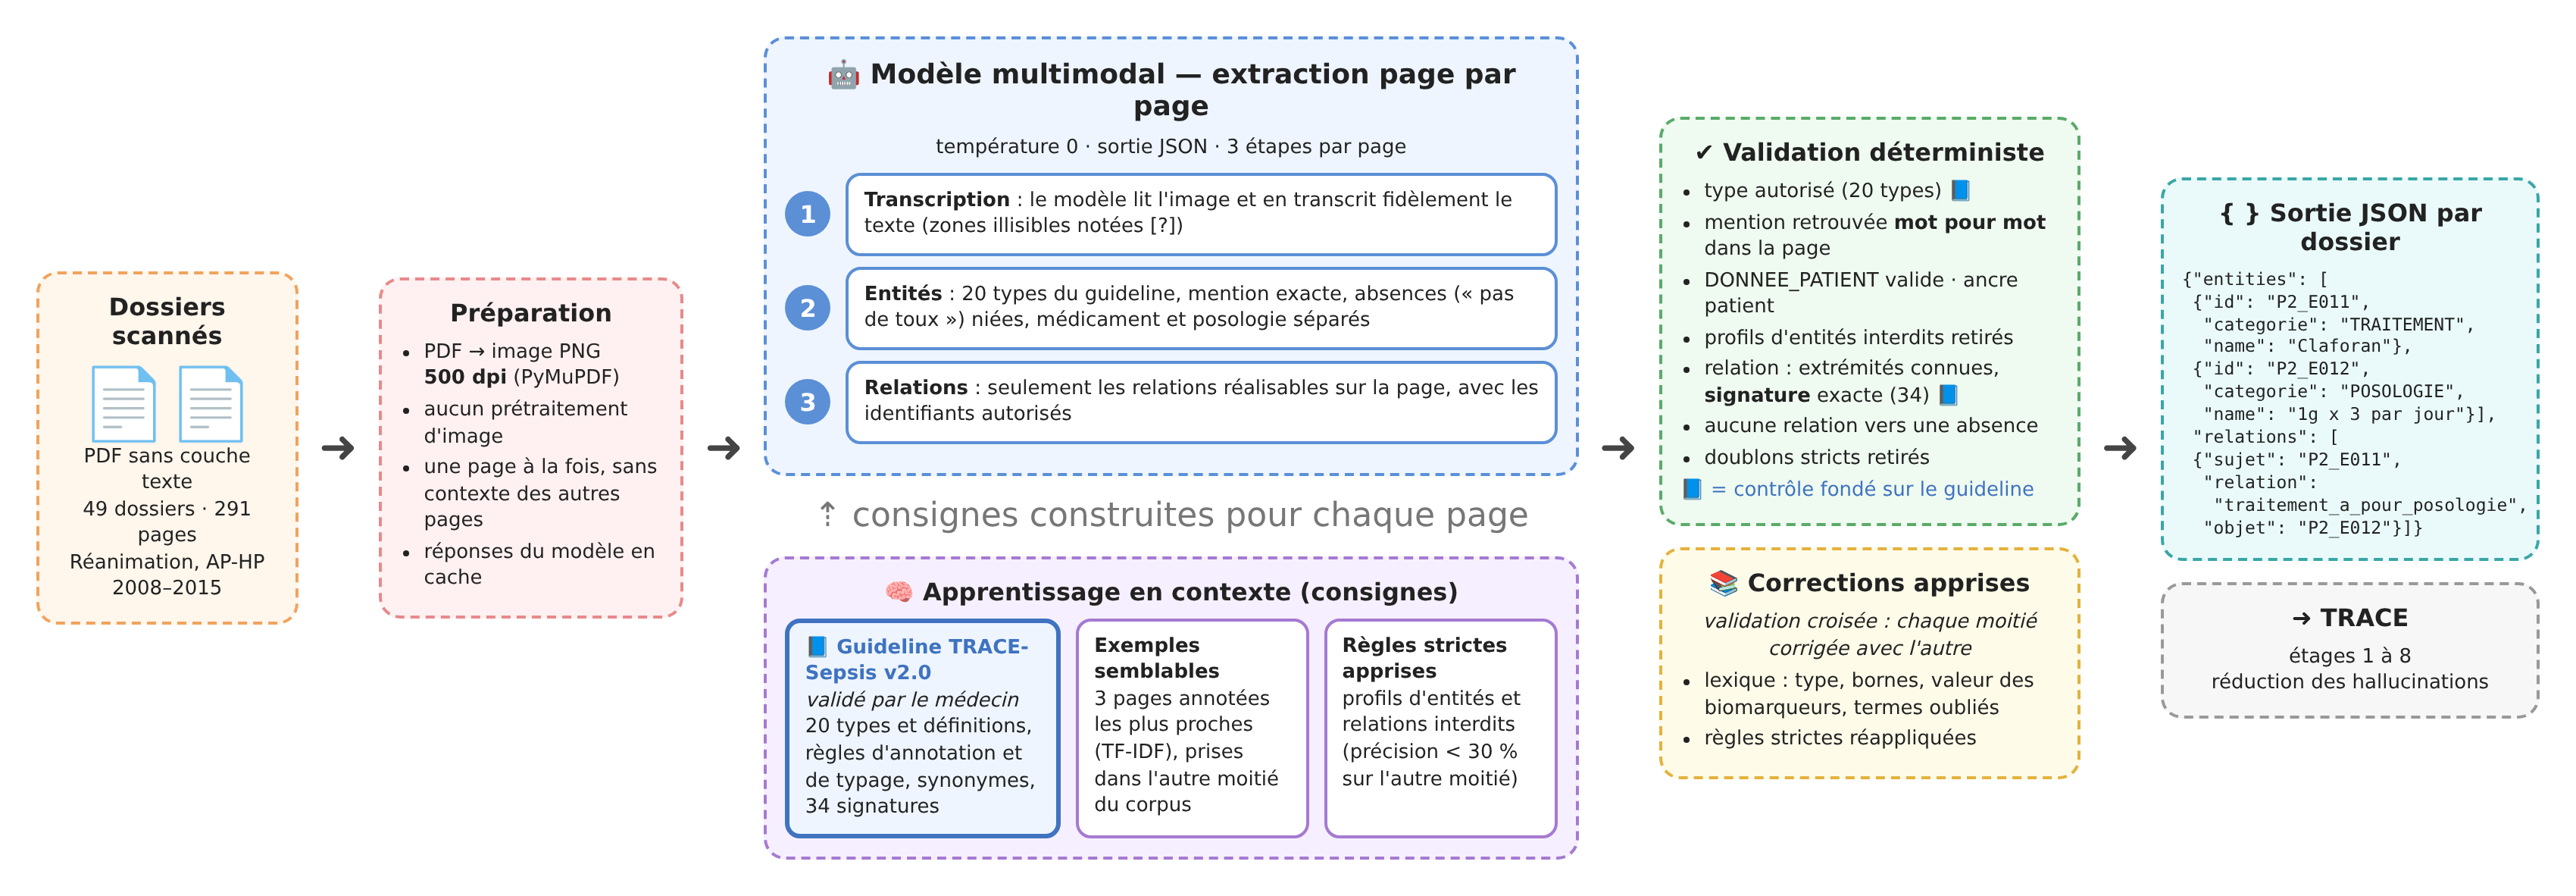
\includegraphics[width=\textwidth]{images/fig_pipeline_extraction.png}
\caption{Pipeline d'extraction multimodale}\label{fig:c4-pipeline}
\end{figure}

La transcription n'est pas un OCR au sens classique : c'est le même modèle multimodal qui lit l'image. Elle fixe une fois pour toutes le texte de la page, sur lequel s'appuient ensuite l'extraction et toutes les vérifications d'ancrage, ici comme dans TRACE. Séparer les entités des relations présente deux autres avantages. Chaque étape porte sur une tâche plus simple, avec une consigne plus courte. Surtout, les relations sont extraites à partir d'une liste d'entités déjà établie et filtrée, ce qui empêche le modèle de relier des éléments qui n'existent pas dans la page.

% ------------------------------------------------------------
\section{Préparation des dossiers médicaux}\label{sec:c4-preparation}

\subsection{Conversion des PDF en images}\label{sec:c4-conversion}

Les dossiers sont des fichiers PDF sans couche texte, obtenus par numérisation de documents papier (section~\ref{sec:c3-3-2-4}). Chaque page est convertie en image PNG à une résolution de 500~dpi, sans canal de transparence, à l'aide de la bibliothèque PyMuPDF. Cette résolution élevée répond à une contrainte connue des MLLMs : leur capacité de lecture se dégrade nettement lorsque la résolution de l'image diminue, au point de passer sous celle d'un OCR classique en dessous d'environ 150~ppi~\cite{inoue2025context}. Une résolution élevée préserve les caractères fins, les indices et les unités, fréquents dans les résultats biologiques et les prescriptions. L'image est transmise au modèle encodée en base64, puis supprimée une fois la page transcrite.

\subsection{Prétraitement}\label{sec:c4-pretraitement}

Aucun prétraitement n'est appliqué aux images : ni redressement, ni débruitage, ni binarisation. Contrairement aux OCR classiques, dont les performances dépendent de ces opérations, les MLLMs reçoivent l'image telle quelle, et une transformation de l'image risquerait de supprimer des détails utiles à la lecture. La contrepartie est que la qualité de la lecture dépend entièrement des capacités visuelles du modèle.

\subsection{Gestion des documents multi-pages}\label{sec:c4-multipages}

Les dossiers comptent de 4 à 12 pages (section~\ref{sec:c3-3-2-3}). Chaque page est soumise au modèle indépendamment des autres : le modèle ne reçoit aucun contexte des pages précédentes. Une relation dont les deux extrémités figurent sur des pages différentes ne peut donc pas être extraite ; cette limite est mesurée par le rappel des relations. Les entités extraites de chaque page reçoivent un identifiant qui indique leur page d'origine (par exemple \texttt{P1\_E015} pour la quinzième entité de la page~1), puis les résultats de toutes les pages sont réunis dans un fichier JSON par dossier. Ce traitement par page reprend le choix fait pour l'annotation du Gold Standard : la page est l'unité de travail, le dossier l'unité de référence (section~\ref{sec:c3-3-7-3}). Il permet aussi d'apparier les entités page par page lors de l'évaluation (section~\ref{sec:c4-matching}).

Toutes les réponses du modèle sont conservées dans un cache, indexé par le contenu exact de la requête. Une interruption ne fait pas perdre le travail déjà fait, et une relance avec les mêmes consignes produit exactement les mêmes sorties.

% ------------------------------------------------------------
\section{Conception des consignes (\emph{prompt engineering})}\label{sec:c4-prompt}

\subsection{Consignes guidées par le guideline}\label{sec:c4-guideline}

Les consignes sont générées automatiquement à partir du fichier du TRACE-Sepsis Annotation Guideline, version~2.0 validée par le médecin. Elles en reprennent les types d'entités avec leurs descriptions et leurs valeurs autorisées, les règles générales d'annotation, les règles de typage (signe vital ou symptôme, diagnostic ou foyer, traitement administré ou envisagé\dots), la table des synonymes, et les 34 relations avec leurs signatures.

Ce choix s'appuie sur deux résultats de la littérature. Pour la reconnaissance d'entités cliniques par un LLM, intégrer des extraits des guidelines d'annotation dans la consigne améliore nettement les performances par rapport à une consigne de base~\cite{hu2024clinicalner}. Plus généralement, un modèle qui reçoit des guidelines détaillées dans sa consigne généralise mieux à de nouveaux schémas d'extraction~\cite{sainz2024gollie}. Il garantit en outre que le modèle et l'annotatrice du Gold Standard suivent les mêmes définitions.

La figure~\ref{fig:c4-prompt} présente la structure d'une consigne d'extraction des entités. Elle se compose de blocs successifs :
\begin{enumerate}
  \item le \textbf{rôle} donné au modèle (expert en extraction d'information clinique sur le sepsis) et la \textbf{mission} (extraire de façon exhaustive les entités explicitement écrites dans la page) ;
  \item les \textbf{règles absolues} : surface exacte, un seul type par mention, aucune inférence, posologie séparée du traitement, mention du patient, absences ;
  \item les \textbf{règles générales}, les \textbf{règles de typage} et les \textbf{synonymes} du guideline ;
  \item les \textbf{définitions} des 20 types d'entités ;
  \item les \textbf{règles strictes apprises} sur l'autre moitié du corpus (section~\ref{sec:c4-regles-strictes}) ;
  \item trois \textbf{exemples annotés}, choisis parmi les pages les plus semblables de l'autre moitié du corpus (section~\ref{sec:c4-exemples}) ;
  \item le \textbf{format de sortie} JSON attendu ;
  \item le \textbf{texte de la page}.
\end{enumerate}
La transcription utilise une consigne à part, volontairement simple : transcrire fidèlement le texte visible, sans résumer, reformuler ni corriger, sans compléter une information absente, en notant \texttt{[?]} une zone illisible et en conservant les abréviations, les retours à la ligne et l'ordre de lecture.

\begin{figure}[H]
\centering
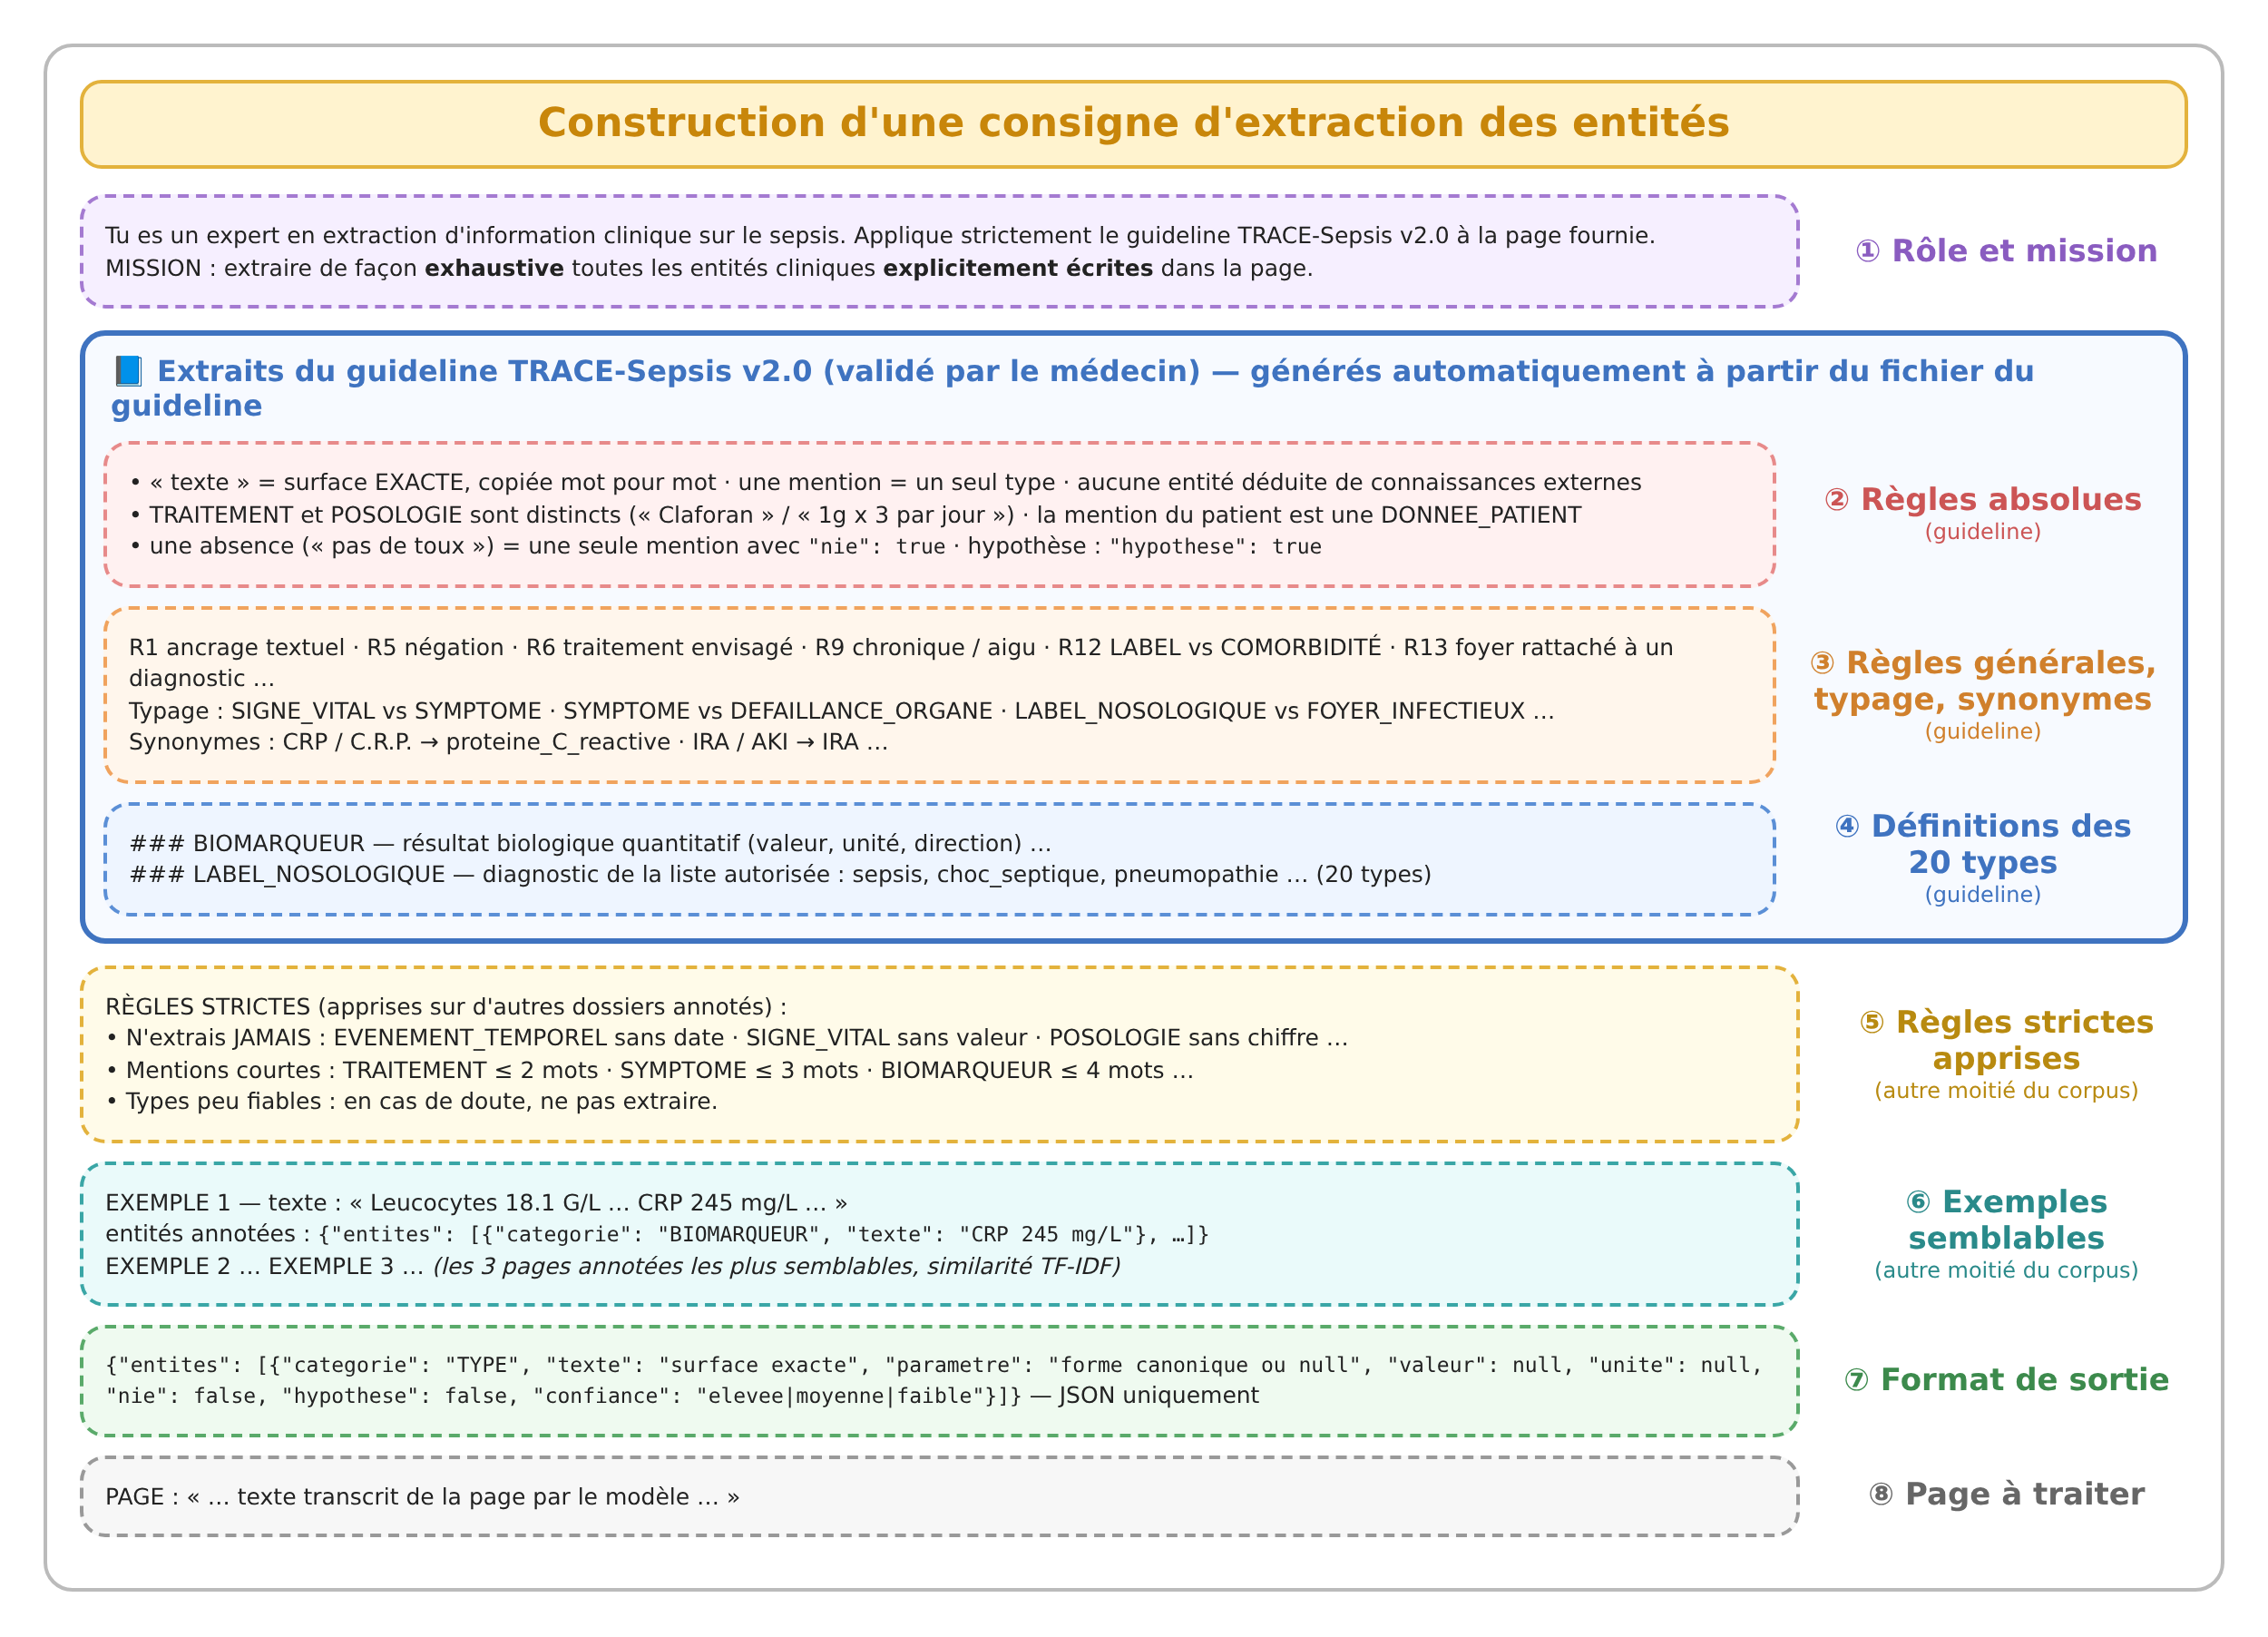
\includegraphics[width=\textwidth]{images/fig_prompt.png}
\caption{Structure d'une consigne d'extraction des entités}\label{fig:c4-prompt}
\end{figure}

\subsection{Exemples annotés choisis par similarité}\label{sec:c4-exemples}

Le modèle n'est pas entraîné sur nos données : ses paramètres restent inchangés. Il apprend la tâche uniquement à partir de ce que contient la consigne, en particulier d'exemples de pages accompagnées de leur annotation. C'est ce que l'on appelle l'apprentissage en contexte (\emph{in-context learning}), dont l'intérêt pour l'extraction d'information clinique a été montré avec peu d'exemples~\cite{agrawal2022fewshot}.

Chaque consigne contient ainsi trois pages annotées du Gold Standard, qui montrent concrètement la convention d'annotation : découpage des mentions, choix du type, posologie séparée du traitement, mention du patient, absences. Ces exemples ne sont pas fixes : pour chaque page à extraire, on retient les trois pages annotées dont le vocabulaire est le plus proche, mesuré par la similarité cosinus de leurs vecteurs TF-IDF. Une page de biologie reçoit ainsi des exemples de biologie, une ordonnance des exemples d'ordonnance. Choisir des exemples proches de la donnée à traiter améliore nettement l'apprentissage en contexte par rapport à des exemples tirés au hasard~\cite{liu2022incontext}.

Pour éviter toute fuite, les exemples sont choisis en validation croisée à deux plis, avec les mêmes plis que l'évaluation de TRACE (dossiers triés, de rang pair et impair) : un dossier ne reçoit que des pages de l'autre moitié du corpus, jamais sa propre annotation. Pour les traitements, l'exemple ne montre que les traitements et posologies annotés ; pour les relations, que les relations annotées.

\subsection{Règles strictes apprises}\label{sec:c4-regles-strictes}

Les consignes contiennent aussi des règles strictes, apprises pour chaque moitié du corpus sur l'autre moitié, en comparant une extraction précédente au Gold Standard. Toute catégorie d'éléments observée au moins cinq fois et dont moins de 30~\% étaient justes est interdite :
\begin{itemize}
  \item des \textbf{profils d'entités}, définis par le type, la présence d'un chiffre et la longueur de la mention (par exemple un événement temporel sans date, un signe vital ou un biomarqueur sans valeur, une posologie sans chiffre) ; une mention niée n'est jamais interdite, car l'absence d'un signe est une information clinique ;
  \item des \textbf{types de relations d'interprétation}, presque toujours faux dans l'extraction précédente (par exemple \emph{biomarqueur\_obtenu\_a}, \emph{precede}, \emph{comorbidite\_est\_facteur\_risque\_de}).
\end{itemize}
Les consignes indiquent aussi la longueur habituelle des mentions de chaque type dans le Gold Standard et signalent les types peu fiables, à n'extraire qu'en cas de correspondance exacte à leur définition. Ces règles sont ensuite réappliquées sans exception lors de la validation (sections~\ref{sec:c4-entites} et~\ref{sec:c4-relations}).

Ces règles, comme les exemples, s'appuient sur la référence pour construire les consignes. C'est pourquoi elles sont systématiquement apprises sur l'autre moitié du corpus : la performance mesurée reste une estimation obtenue sur des dossiers dont l'annotation n'a pas servi à guider l'extraction. Ce guide appris ne contient aucun texte de dossier, seulement des types, des profils et des taux.

\subsection{Contraintes sur les entités}\label{sec:c4-contraintes-entites}

La consigne d'extraction des entités impose les règles suivantes :
\begin{itemize}
  \item seuls les 20 types d'entités du schéma sont autorisés, et chaque mention reçoit un seul type ;
  \item la mention est recopiée telle qu'elle apparaît dans la page, sous sa forme autonome la plus courte, sans reformulation ;
  \item aucune information absente de la page ne doit être ajoutée, même médicalement plausible ;
  \item une pneumopathie, un abcès, une pyélonéphrite, un érysipèle ou une sinusite sont des diagnostics (\entite{LABEL\_NOSOLOGIQUE}) ; \entite{FOYER\_INFECTIEUX} ne désigne que leur localisation ;
  \item \entite{TRAITEMENT} et \entite{POSOLOGIE} sont deux entités distinctes : le traitement est le nom seul du médicament, la dose, le schéma, la voie et la durée forment la posologie ; les listes d'ordonnance (traitement habituel, traitement de sortie) sont aussi extraites ;
  \item chaque mention qui désigne le patient (\og le patient \fg{}, \og la patiente de 77 ans \fg{}) est une entité \entite{DONNEE\_PATIENT}, jamais un titre de section ni un examen ;
  \item une absence (\og pas de toux \fg{}) est une seule mention couvrant la proposition niée, signalée par l'indicateur \emph{nie} ; une hypothèse est signalée par l'indicateur \emph{hypothese} ;
  \item les synonymes et abréviations sont reconnus et ramenés à une forme canonique, stockée à part ;
  \item aucune donnée directement identifiante n'est extraite.
\end{itemize}
Avec la seule consigne générale, le modèle rattachait souvent la posologie au nom du médicament (\og Claforan, 1g x 3 par jour \fg{} extrait comme un seul traitement). L'étape des entités comporte donc une seconde passe, limitée aux médicaments : une consigne courte reprend les définitions de \entite{TRAITEMENT} et \entite{POSOLOGIE} du guideline et demande d'extraire séparément chaque médicament d'une ligne qui en cite plusieurs ; ses entités remplacent les traitements et posologies de la première passe.

\subsection{Contraintes sur les relations}\label{sec:c4-contraintes-relations}

La consigne d'extraction des relations fournit au modèle le texte de la page et la liste des entités conservées, classées par type, et impose les règles suivantes :
\begin{itemize}
  \item seules les relations réalisables sur la page sont proposées, c'est-à-dire celles pour lesquelles il existe au moins une entité du type attendu comme sujet et une comme objet ; pour chacune, la consigne donne la liste des identifiants autorisés de part et d'autre ;
  \item les relations interdites par les règles strictes apprises ne sont pas proposées ;
  \item une relation relie deux entités de la liste, désignées par leur identifiant, et n'est jamais inversée pour devenir valide ;
  \item une relation doit être énoncée par une phrase de la page, et non déduite de la seule présence de deux entités ;
  \item aucune relation ne pointe vers une absence ;
  \item un traitement seulement envisagé ne reçoit pas de relation \emph{traitement\_administre\_a}.
\end{itemize}
Restreindre explicitement les candidats répond à une erreur fréquente lors des premiers essais : le modèle choisissait le bon type de relation mais l'orientait vers une entité d'un autre type, par exemple une administration de traitement dirigée vers un biomarqueur plutôt que vers le patient. Sur un dossier d'essai, le nombre de relations rejetées par la validation pour non-respect de la signature est passé de 74 à 5 après cette modification. Lorsqu'aucune relation n'est réalisable sur une page, l'appel au modèle n'est pas effectué.

\subsection{Format JSON structuré}\label{sec:c4-json}

Chaque appel doit renvoyer un objet JSON conforme à un format fixé dans la consigne, et l'appel active le mode JSON de l'API. Une entité comporte son type, sa mention, sa forme canonique, sa valeur et son unité éventuelles, les indicateurs de négation (\emph{nie}) et d'hypothèse, un niveau de confiance (élevée, moyenne ou faible) et le type d'inférence ; après validation, elle reçoit un identifiant, sa page et sa position dans le texte. Une relation comporte les identifiants de son sujet et de son objet, son type, sa preuve textuelle et un niveau de confiance. Ces champs correspondent aux métadonnées de traçabilité prévues par le guideline (section~\ref{sec:c3-3-4-2}). La figure~\ref{fig:c4-json} en donne un exemple, construit pour l'illustration.

\begin{figure}[H]
\centering
\begin{minipage}{0.92\linewidth}
\footnotesize
\begin{verbatim}
{"entities": [
  {"identifiant_entite": "P2_E004", "categorie": "BIOMARQUEUR",
   "name": "CRP 245 mg/L", "parametre": "proteine_C_reactive",
   "valeur": "245", "unite": "mg/L", "nie": false, "confiance": "elevee",
   "page": 2, "start": 812, "end": 824},
  {"identifiant_entite": "P2_E011", "categorie": "TRAITEMENT",
   "name": "Claforan", "nie": false, "confiance": "elevee", "page": 2},
  {"identifiant_entite": "P2_E012", "categorie": "POSOLOGIE",
   "name": "1g x 3 par jour", "nie": false, "confiance": "elevee", "page": 2}],
 "relations": [
  {"identifiant_entite_sujet": "P2_E011",
   "type_relation": "traitement_a_pour_posologie",
   "identifiant_entite_objet": "P2_E012",
   "preuve": "Claforan 1g x 3 par jour", "confiance": "elevee"}]}
\end{verbatim}
\end{minipage}
\caption{Exemple de sortie JSON d'une page (exemple construit, sans donnée patient)}\label{fig:c4-json}
\end{figure}

Imposer un format structuré a deux intérêts. La sortie peut être lue automatiquement, sans interprétation d'un texte libre. Chaque élément porte sa page, sa position et, pour les relations, sa preuve, ce qui permet de vérifier ensuite qu'il provient bien du document : cette traçabilité est la base des vérifications de TRACE.

Tous les appels sont faits à température~0, afin que le modèle choisisse à chaque pas la réponse la plus probable et que l'extraction soit reproductible.

% ------------------------------------------------------------
\section{Modèles multimodaux évalués}\label{sec:c4-modeles}

Deux modèles multimodaux ont été comparés. Tous deux acceptent en entrée une image et une consigne textuelle, et ont été choisis parce qu'ils peuvent être utilisés dans des conditions compatibles avec la protection des données de santé (section~\ref{sec:c3-3-2-4}).

\subsection{Qwen2.5-VL}\label{sec:c4-qwen}

Qwen2.5-VL~\cite{bai2025qwen25vl} est un modèle vision-langage à poids ouverts. Il figure parmi les modèles compacts qui obtiennent les meilleurs taux d'erreur de transcription face aux OCR classiques et neuronaux sur des comptes rendus médicaux photographiés~\cite{neveditsin2026compact}. Nous avons utilisé sa version à 7~milliards de paramètres ajustée pour suivre des instructions, Qwen2.5-VL-7B-Instruct, exécutée localement sur un GPU de l'infrastructure de l'université, à température~0. Les conditions de protection des données sont décrites à la section~\ref{sec:c3-3-2-4}.

\subsection{Mistral Small 4}\label{sec:c4-mistral}

Mistral Small 4 (\texttt{mistral-small-2603})~\cite{mistralsmall4} réunit dans un seul modèle des capacités de vision, de raisonnement et de génération, et accepte en entrée du texte et des images. Il a été utilisé par l'intermédiaire de l'offre payante de l'API de Mistral AI, à température~0, dans les conditions de protection des données décrites à la section~\ref{sec:c3-3-2-4}.

\subsection{Protocole comparatif}\label{sec:c4-protocole}

Pour que la comparaison soit équitable, les deux modèles ont été évalués avec exactement le même pipeline (figure~\ref{fig:c4-pipeline}) :
\begin{itemize}
  \item les mêmes 49 dossiers, convertis en images de la même façon ;
  \item les mêmes trois étapes par page (transcription, entités, relations) et les mêmes consignes, avec des exemples semblables et des règles strictes construits de la même manière et sur les mêmes plis ;
  \item la même validation déterministe et les mêmes corrections apprises sur le Gold Standard ;
  \item la même évaluation, contre le même Gold Standard, avec les mêmes modes d'appariement et les mêmes métriques (chapitre~\ref{chap:donnees-gold}, sections~\ref{sec:c4-matching} et~\ref{sec:c4-metriques}).
\end{itemize}
Les paramètres de génération sont eux aussi identiques : température~0 pour tous les appels, et une même longueur maximale de réponse pour chaque étape, de 4\,000~jetons pour la transcription, 8\,000 pour les entités et les relations, et 12\,000 pour la seconde passe sur les médicaments. Seul le modèle change, ainsi que ses conditions d'exécution : Qwen2.5-VL est exécuté localement sur le GPU de l'université, Mistral Small~4 par l'API de Mistral AI.

% ------------------------------------------------------------
\section{Extraction des entités}\label{sec:c4-entites}

Pour chaque page, le modèle reçoit le texte transcrit et la consigne d'extraction des entités (section~\ref{sec:c4-contraintes-entites}), complétée par la seconde passe sur les médicaments ; il renvoie la liste des entités au format JSON. Chaque entité renvoyée est ensuite contrôlée de façon déterministe :
\begin{enumerate}
  \item \textbf{type autorisé} : son type doit faire partie des 20 types du guideline ;
  \item \textbf{ancrage dans la page} : sa mention doit être retrouvée dans le texte de la page, sans tenir compte de la casse ni des espaces ; c'est la surface trouvée dans la page qui est conservée, avec sa position ; une mention répétée (\og 1-0-0 \fg{} sur chaque ligne d'ordonnance) est rattachée à l'occurrence suivante encore libre ;
  \item \textbf{patient} : une entité \entite{DONNEE\_PATIENT} doit désigner le patient ou porter une donnée démographique (âge, sexe, poids\dots) ; un titre comme \og Sur le plan rénal \fg{} est écarté ;
  \item \textbf{règles strictes apprises} : une entité d'un profil interdit est écartée ;
  \item \textbf{unicité} : deux entités de même position sont fusionnées.
\end{enumerate}
Enfin, si la page nomme le patient sans qu'aucune entité ne le désigne, la première mention (\og la patiente de 77 ans \fg{}) devient l'entité patient de la page. Cette règle déterministe ne crée aucune information clinique ; elle fournit l'extrémité nécessaire aux relations du patient (diagnostic, traitement administré, symptôme, défaillance).

Le contrôle d'ancrage écarte dès l'extraction les entités inventées ou reformulées, c'est-à-dire la forme la plus directe d'hallucination factuelle. Il ne protège pas contre une erreur de transcription : une valeur mal lue puis recopiée à l'identique sera ancrée dans une transcription elle-même fausse ; ce cas relève des hallucinations visuelles.

% ------------------------------------------------------------
\section{Extraction des relations}\label{sec:c4-relations}

Le modèle reçoit ensuite le texte de la page, la liste des entités conservées et la consigne d'extraction des relations (section~\ref{sec:c4-contraintes-relations}). Il renvoie la liste des relations, chacune désignant son sujet et son objet par leur identifiant.

Chaque relation est confrontée au schéma : elle n'est conservée que si ses deux extrémités sont des entités de la page, si son type fait partie des 34 relations autorisées et si les types de son sujet et de son objet correspondent exactement à sa signature, ce qui exclut une relation inversée. Sont aussi écartées les relations d'un type interdit par les règles strictes apprises et les relations dont une extrémité est une absence. Un même triplet n'est gardé qu'une fois. Les relations écartées sont conservées à part, avec le motif du rejet, pour l'analyse des erreurs.

% ------------------------------------------------------------
\section{Mise en forme des sorties}\label{sec:c4-postproc}

La mise en forme décrite ici se limite à ce qui est nécessaire pour obtenir un fichier exploitable. Les vérifications destinées à réduire les hallucinations relèvent des étages suivants de TRACE (chapitre~\ref{chap:architecture}).

\subsection{Normalisation JSON}\label{sec:c4-norm-json}

Une sortie de modèle génératif n'est pas toujours un JSON valide, même avec le mode JSON : balises de code, texte ajouté avant ou après l'objet. Le pipeline retire ces balises, tente de lire la réponse entière comme un objet JSON puis, en cas d'échec, le premier bloc entre accolades. Une réponse illisible est remplacée par une sortie vide pour la page concernée, plutôt que d'interrompre le traitement ; aucune nouvelle requête n'est faite. En cas d'erreur réseau ou de limite de débit de l'API, la requête est relancée jusqu'à quinze fois avec un délai croissant. Les noms de types sont normalisés (majuscules, variantes comme \texttt{SCORE\_QSOFA}) et les champs manquants reçoivent une valeur par défaut.

\subsection{Nettoyage des entités}\label{sec:c4-nettoyage-entites}

Les entités dont le type ne fait pas partie des 20 types du schéma, dont la mention est vide ou n'est pas retrouvée dans la page sont écartées, ainsi que les entités patient invalides et celles des profils interdits (section~\ref{sec:c4-entites}). La forme canonique proposée par le modèle est conservée à part et ne modifie jamais la mention.

\subsection{Nettoyage des relations}\label{sec:c4-nettoyage-relations}

Les relations dont le type ne fait pas partie du schéma, dont une extrémité est absente ou dont la signature n'est pas respectée sont écartées, comme indiqué à la section~\ref{sec:c4-relations}. Pour chaque relation gardée, le texte du sujet et de l'objet est recopié à côté de leurs identifiants.

\subsection{Gestion des doublons}\label{sec:c4-doublons}

À ce stade, seuls les doublons strictement identiques au sein d'une même page sont retirés : même position pour une entité, même triplet pour une relation. Le traitement des répétitions d'un même fait sur plusieurs pages, plus délicat parce qu'une répétition peut être cliniquement significative (deux dosages successifs d'un même biomarqueur), est réalisé par l'étage de dédoublonnage de TRACE (chapitre~\ref{chap:architecture}).

% ------------------------------------------------------------
\section{Corrections apprises sur le Gold Standard}\label{sec:c4-appris}

Avant d'entrer dans TRACE, la sortie de l'extraction passe par deux corrections déterministes, apprises sur le Gold Standard en validation croisée (chaque moitié du corpus est corrigée avec ce qui est appris sur l'autre) :
\begin{itemize}
  \item un \textbf{lexique} des mentions annotées et de leur type. Une mention vue au moins deux fois et annotée avec un même type dans au moins 80~\% des cas prend ce type ; une mention trop longue qui contient un terme du lexique de même type est recadrée sur ce terme ; un biomarqueur extrait sans valeur reçoit la valeur et l'unité écrites juste après (\og Urée \fg{} devient \og Urée 33 mmol/L \fg{}), conformément à la convention du guideline ; enfin, un terme très fiable (annoté avec ce type dans au moins 80~\% de ses occurrences) et oublié par le modèle est ajouté là où il est écrit dans la page ;
  \item les \textbf{règles strictes} de la section~\ref{sec:c4-regles-strictes}, réappliquées à la sortie : profils d'entités et types de relations dont la précision était inférieure au seuil sur l'autre moitié.
\end{itemize}
Une mention niée n'est jamais modifiée ni retirée par ces corrections. Toutes sont déterministes et ancrées dans le texte : elles ne peuvent ajouter qu'un terme effectivement écrit dans la page, jamais une information absente du document.

% ------------------------------------------------------------
\section{Critères de sélection du modèle d'extraction}\label{sec:c4-selection}

Les deux modèles sont comparés sur la sortie du pipeline d'extraction, avant TRACE, avec le protocole de la section~\ref{sec:c4-protocole}. La comparaison repose sur trois critères, fixés avant l'expérience :
\begin{itemize}
  \item la qualité de l'extraction des \textbf{relations}, mesurée par le F1-score en mode Relaxed et en micro-moyenne, critère principal parce que la valeur d'un graphe de connaissances dépend directement de ses relations : un graphe dont les entités sont justes mais mal reliées ne permet pas de reconstituer le parcours du patient ;
  \item la qualité de l'extraction des \textbf{entités}, mesurée de la même façon ;
  \item le \textbf{taux d'hallucination} des entités et des relations, qui indique la part des éléments extraits que la référence ne justifie pas.
\end{itemize}
Les modes Strict et Boundary-Relaxed et la macro-moyenne servent à vérifier que la conclusion ne dépend pas du mode d'appariement ni de quelques dossiers. Les conditions d'exécution entrent aussi en compte : Qwen2.5-VL tourne sur l'infrastructure de l'université, tandis que Mistral Small~4 passe par une API externe.

Les résultats de cette comparaison, mesurés avec les modes d'appariement et les métriques du chapitre~\ref{chap:donnees-gold}, sont présentés au chapitre~\ref{chap:experimentations}. Le modèle retenu fournit l'extraction à partir de laquelle TRACE est évaluée : chaque étage de la chaîne est mesuré par rapport à cette sortie de départ.

% ------------------------------------------------------------
\section{Conclusion}\label{sec:c4-conclusion}

Ce chapitre a présenté les deux fondements de l'extraction. Le TRACE-Sepsis Annotation Guideline, validé par le médecin, définit 20 types d'entités, 34 relations et les règles qui garantissent une représentation cohérente et fidèle des dossiers. Le pipeline d'extraction fait lire directement les pages scannées par un modèle multimodal, qui en transcrit le texte, puis en extrait les entités et les relations. Ses consignes sont générées à partir du guideline et complétées par des exemples semblables et des règles strictes, appris en validation croisée ; des contrôles déterministes écartent dès l'extraction les entités absentes de la page et les relations hors du schéma. Les deux modèles comparés, Qwen2.5-VL et Mistral Small~4, suivent exactement le même pipeline.

Pour mesurer la qualité de cette extraction, il faut une référence construite sans l'aide des modèles évalués. Le chapitre suivant présente le Gold Standard, son protocole d'annotation, sa validation médicale et la manière dont une extraction lui est comparée.
